% header
\documentclass[10pt,a4paper]{article}

\usepackage[utf8]{inputenc}
\usepackage{hyperref}
\usepackage{amssymb}
\usepackage{amsmath}
\usepackage{listings}
\usepackage{graphicx}

% the document
\begin{document}

\title{Worksheet $3$\\
\small{Practical Lab Numerical Computing}}
\author{Andrii Lischishin \and Lars Schleithoff \and Hendrik Kleikamp}
\date{\today}
\maketitle

\section*{Task 3}

\begin{center}
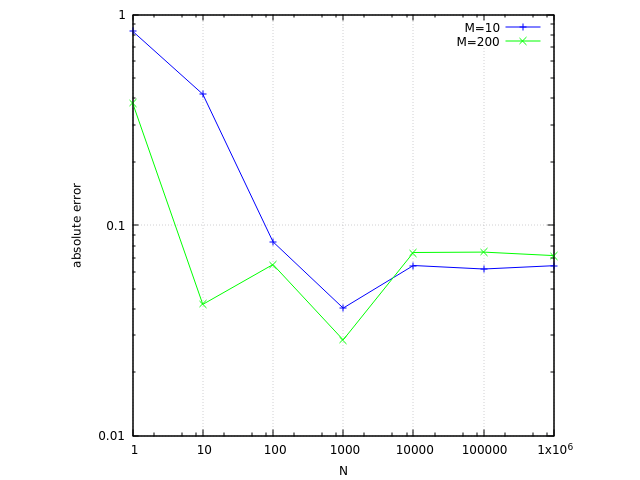
\includegraphics[scale=0.5]{error_task_3.png}
\end{center}
The number of timesteps is not really effecting the convergence.

\section*{Task 4}

\begin{center}
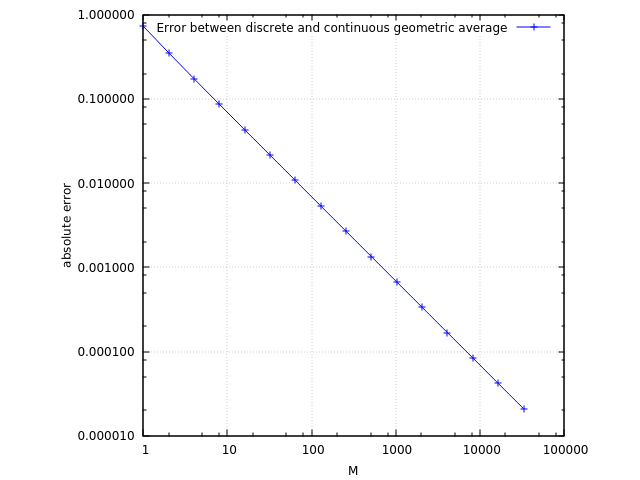
\includegraphics[scale=0.5]{error_continuous_discrete.png}		
\end{center}
The discrete geometric average converges linearly to the continuous geometric average.

\section*{Task 5}

\begin{center}
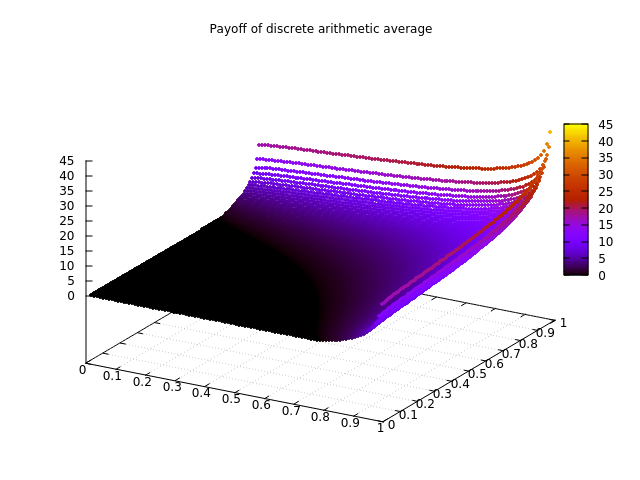
\includegraphics[scale=0.5]{payoff_discrete_arithmetic_average.png}
\end{center}
The discrete geometric payoff function is evaluated on 10.000 points in $[0,1]^2$.

\section*{Task 7}

Uniform random numbers in $(0,1)^2$:
\begin{center}
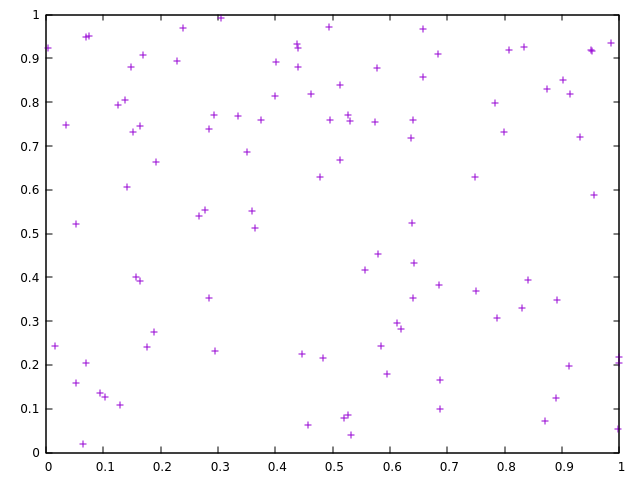
\includegraphics[scale=0.5]{uniform_random_numbers.png}		
\end{center}

Halton sequence:
\begin{center}
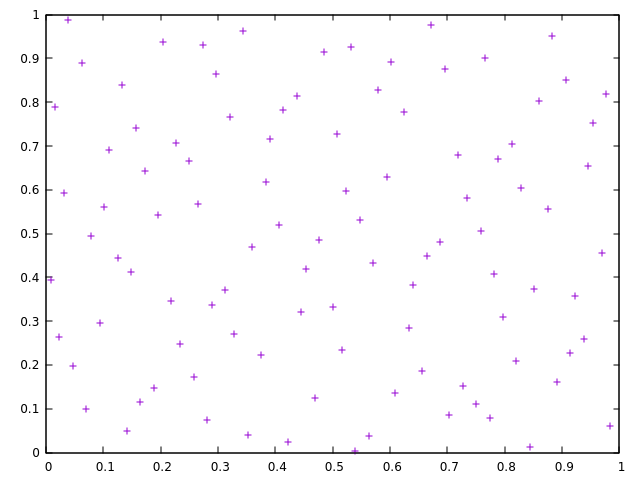
\includegraphics[scale=0.5]{halton_sequence.png}		
\end{center}

One can see that there are some regions in $(0,1)^2$ where no uniform random numbers are set. This is not the case in the point set calculated by the Halton sequence. The Halton sequence gives a very uniform spread set without any holes.

\section*{Task 9}

Quadrature nodes of the two-dimensional product rule for trapezoidal rule:
\begin{center}
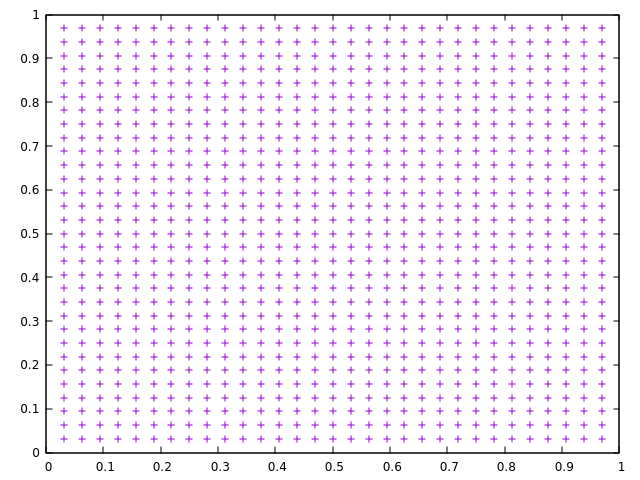
\includegraphics[scale=0.5]{quadrature_nodes_trapezoidal_rule.png}		
\end{center}

Quadrature nodes of the two-dimensional product rule for Gauss-Legendre:
\begin{center}
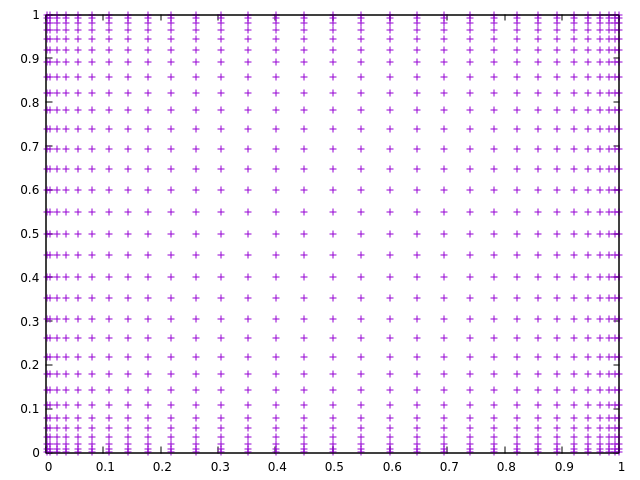
\includegraphics[scale=0.5]{quadrature_nodes_gauss_legendre.png}		
\end{center}

Quadrature nodes of the two-dimensional product rule for Clenshaw Curtis:
\begin{center}
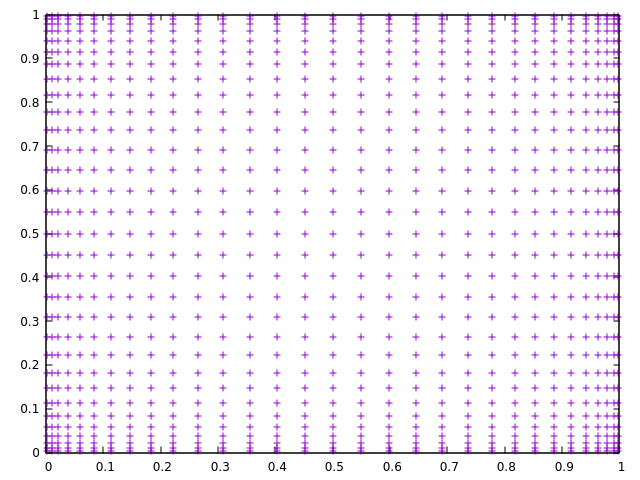
\includegraphics[scale=0.5]{quadrature_nodes_clenshaw_curtis.png}		
\end{center}

Both Gauß-Quadrature and Clenshaw-Curtis-Quadrature have an increased amount of nodes at the edges of the integration region. The trapeziodal rule distributes the nodes equidistantly over the integration region.

\section*{Task 11}

Two-dimensional Sparse Grid using Trapeziodal Rule for $l=5$:
\begin{center}
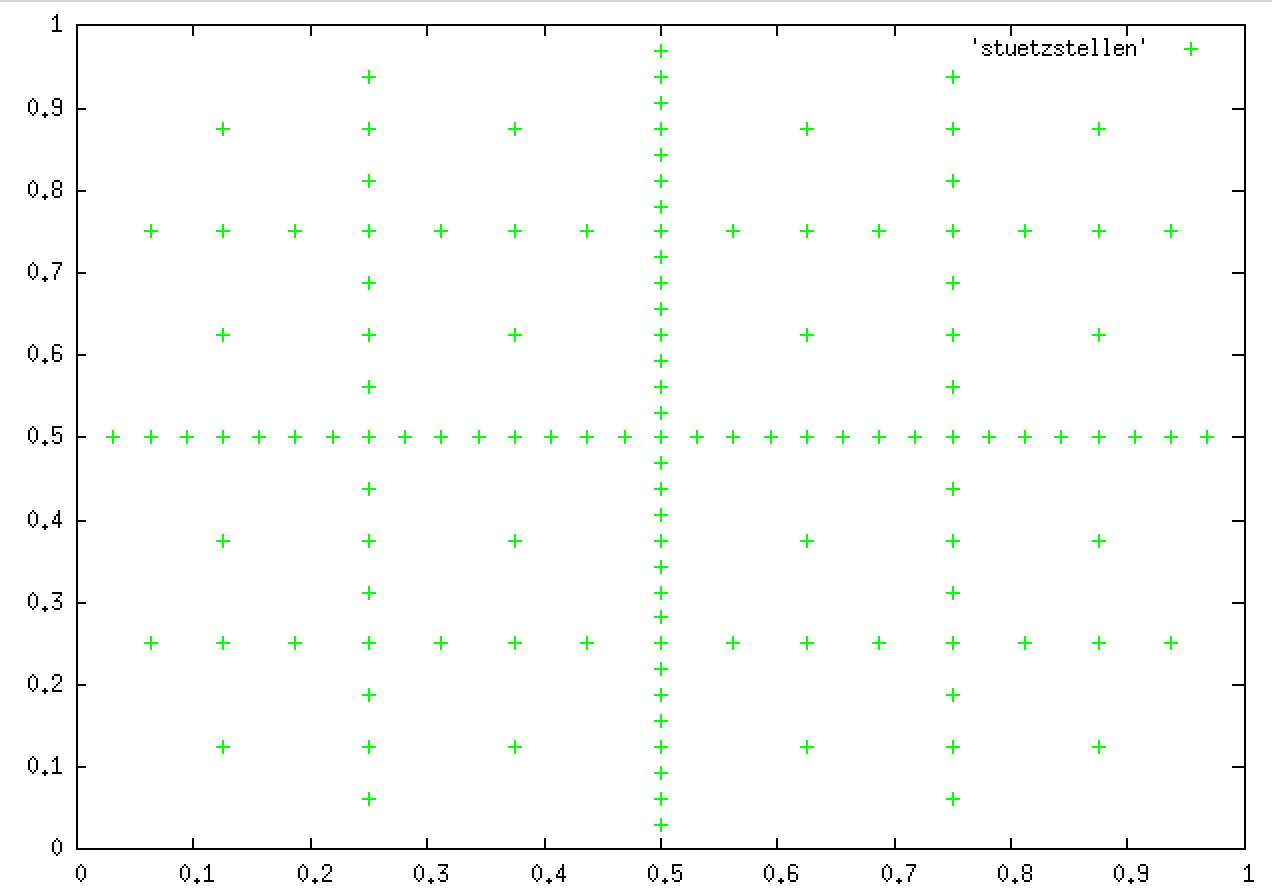
\includegraphics[scale=0.5]{sparse_grid_l5.png}	
\end{center}

Two-dimensional Sparse Grid using Trapezoidal Rule for $l=7$:
\begin{center}
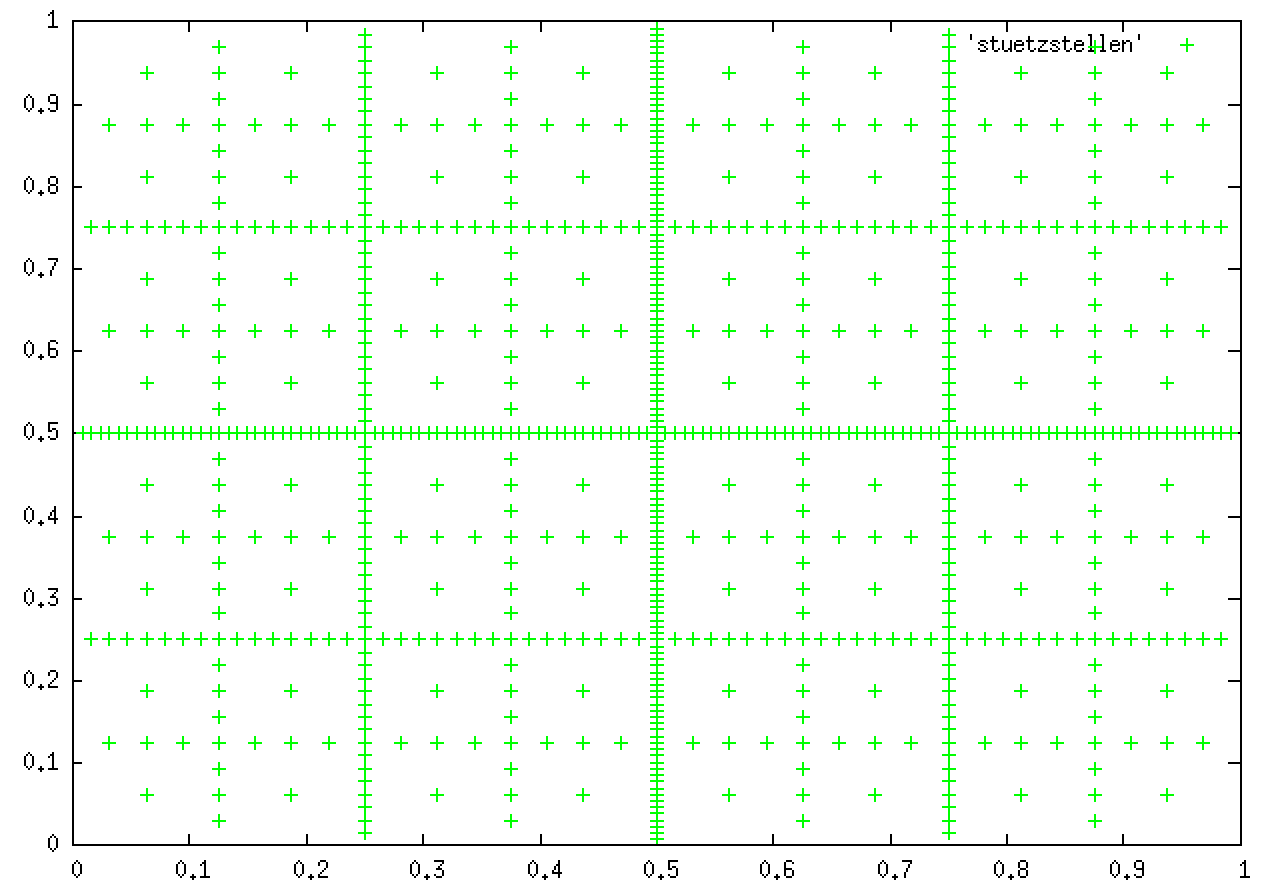
\includegraphics[scale=0.5]{sparse_grid_l7.png}	
\end{center}

Two-dimensional Sparse Grid using Clenshaw-Curtis Quadrature Rule for $l=5$:
\begin{center}
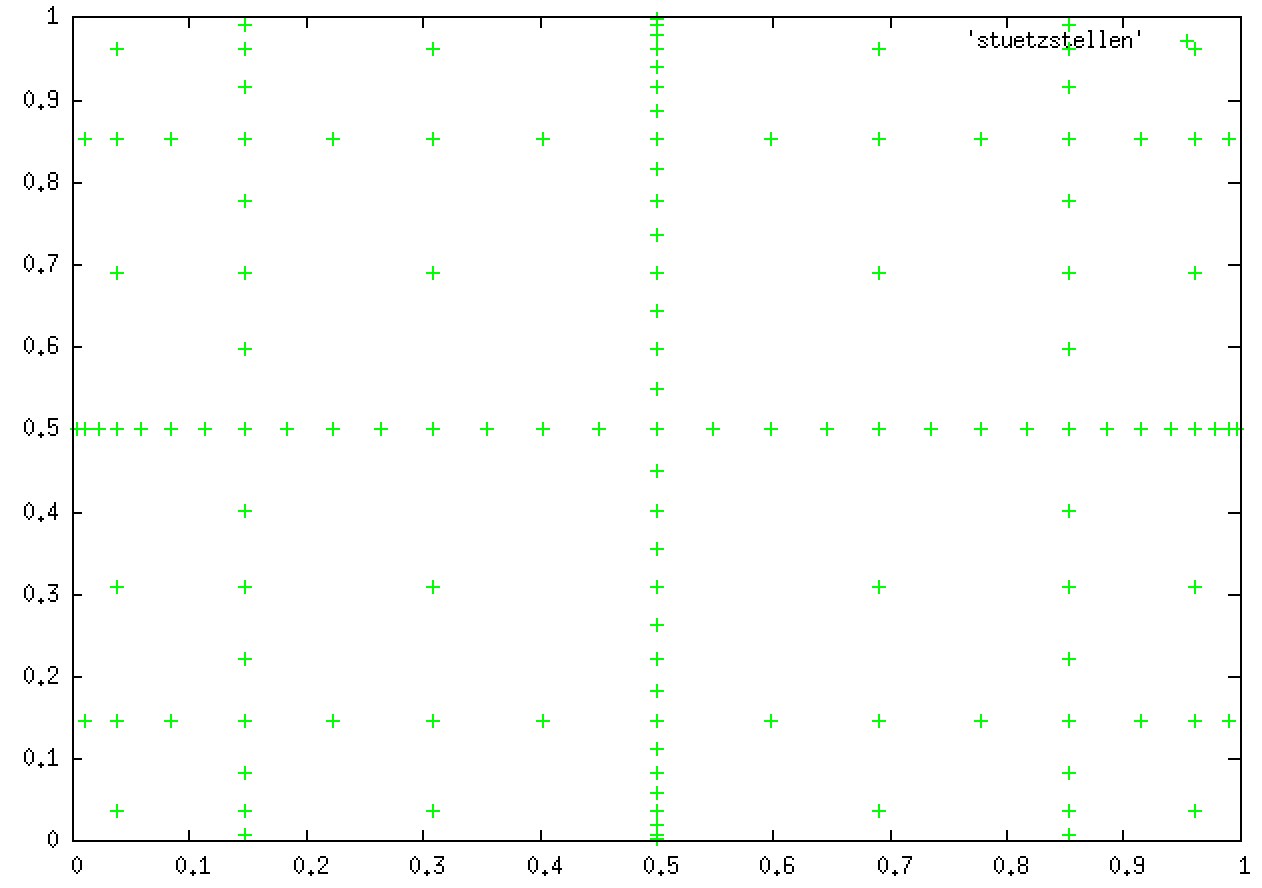
\includegraphics[scale=0.5]{clenshaw_curtis_l5.png}	
\end{center}

Two-dimensional Sparse Grid using Clenshaw-Curtis Quadrature Rule for $l=7$:
\begin{center}
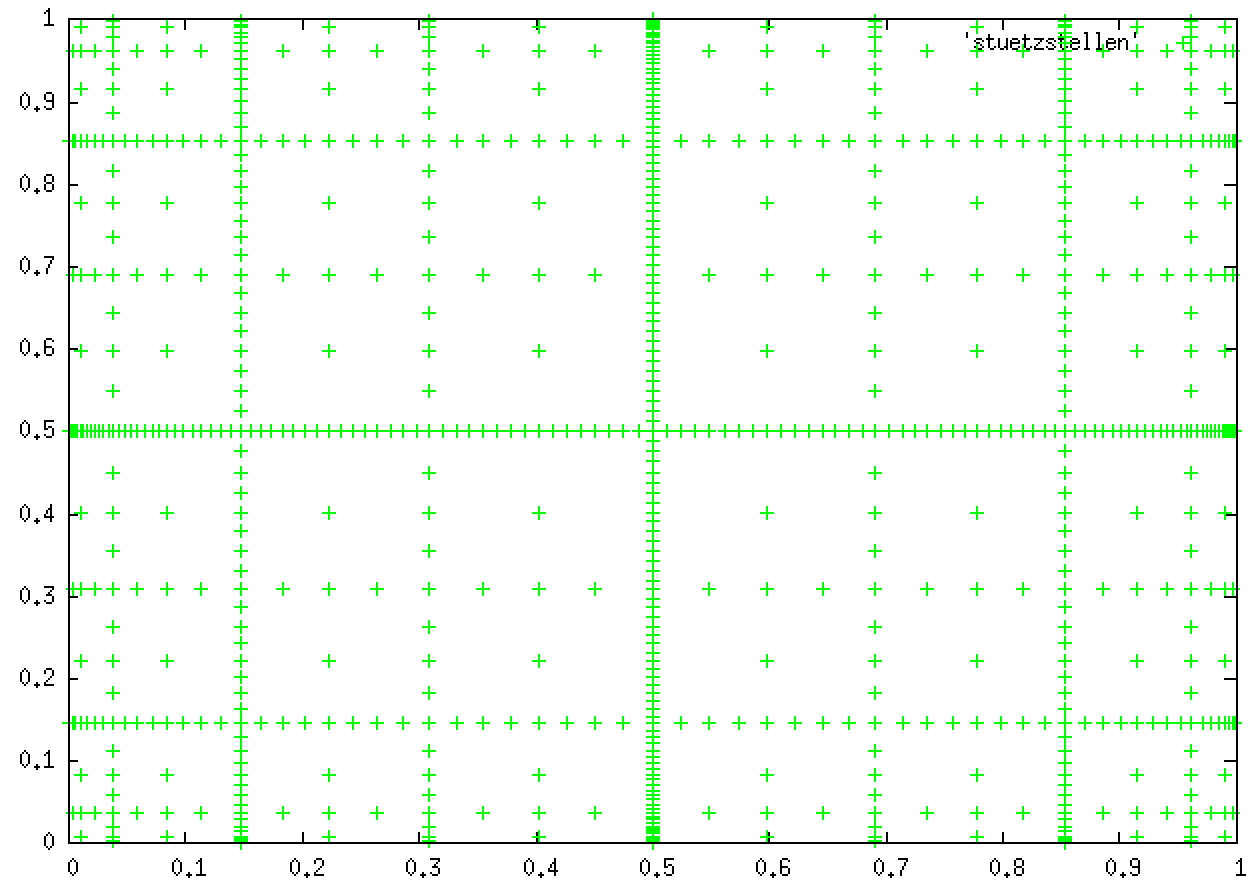
\includegraphics[scale=0.5]{clenshaw_curtis_l7.png}	
\end{center}
For Clenshaw-Curtis Quadrature, with increasing level, more nodes are situated at the edges of the integration region. For Trapezoidal Rule, this is not the case.

\section*{Task 12}

Number of points in Sparse Grid and Full Grid in Level $l=4$:
\begin{center}
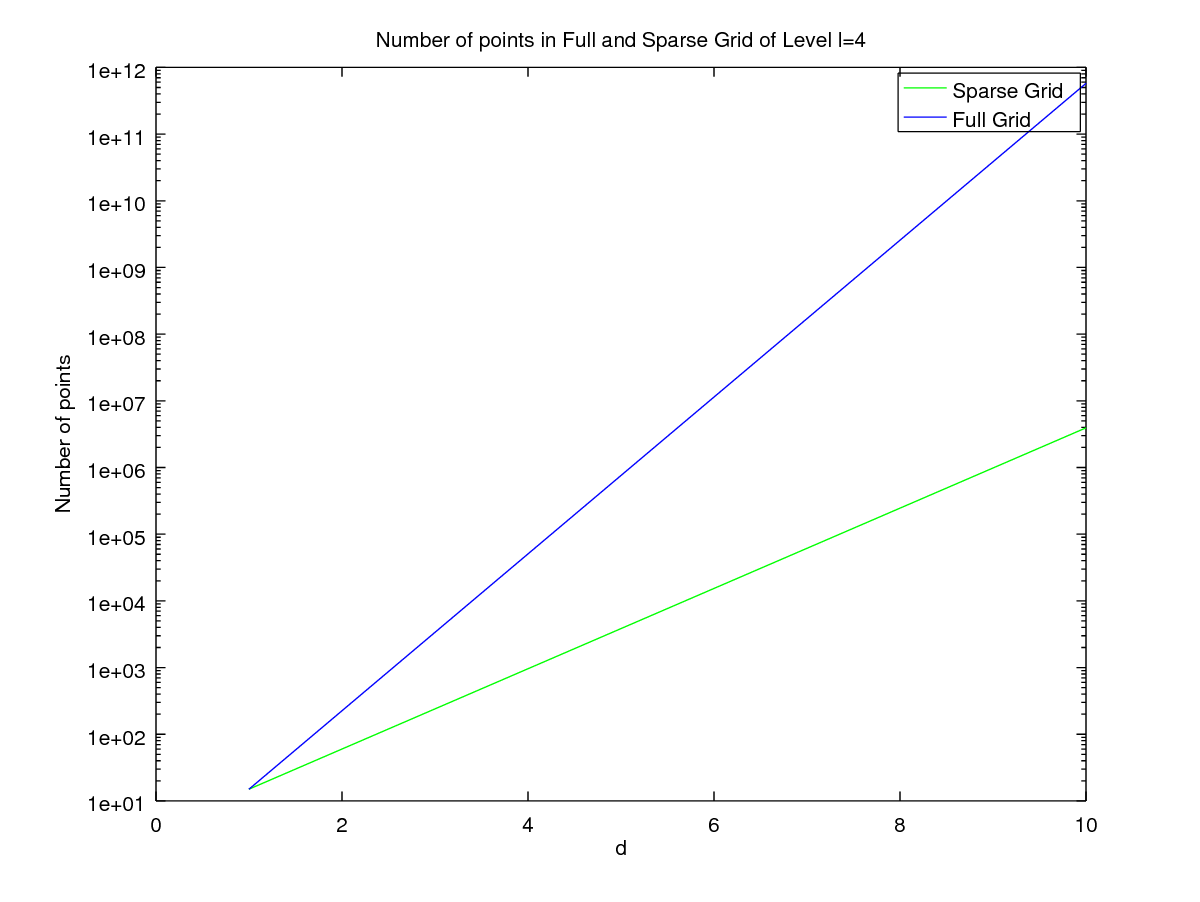
\includegraphics[scale=0.5]{number_of_points_SG_FG.png}
\end{center}
One can see that the number of points increases much faster in the Full Grid, then in the Sparse Grid.

\section*{Task 13}

Convergence plots for the testfunction $f_\gamma$ in different dimensions:
\begin{center}
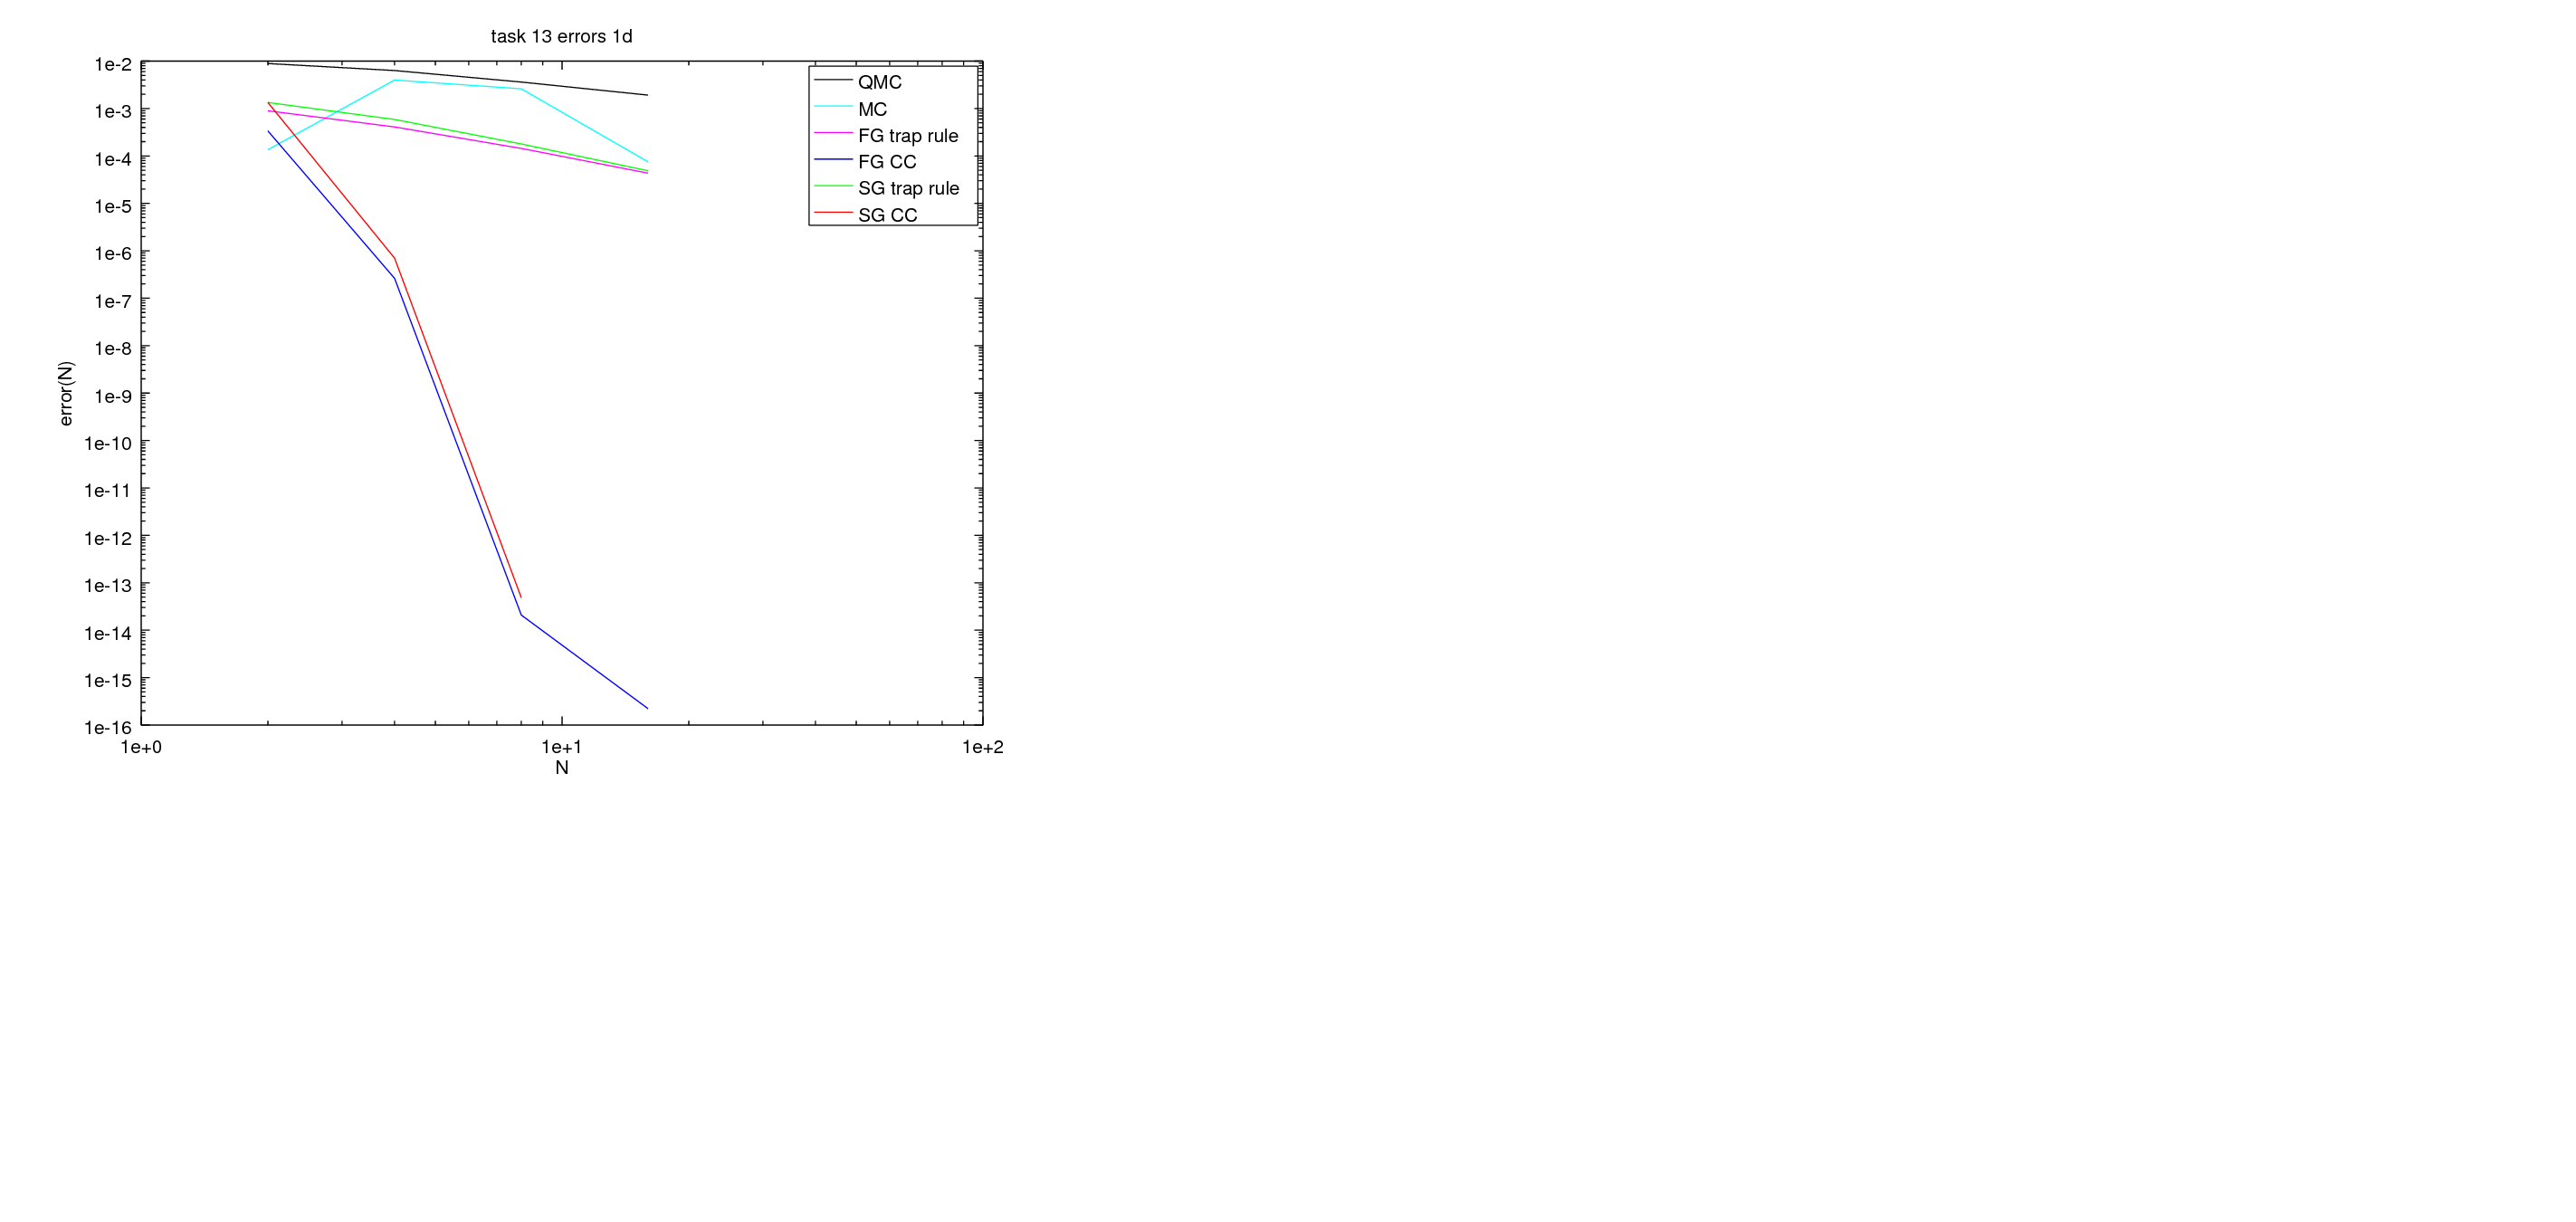
\includegraphics[scale=0.5]{task_13_d1.png}
\end{center}
\begin{center}
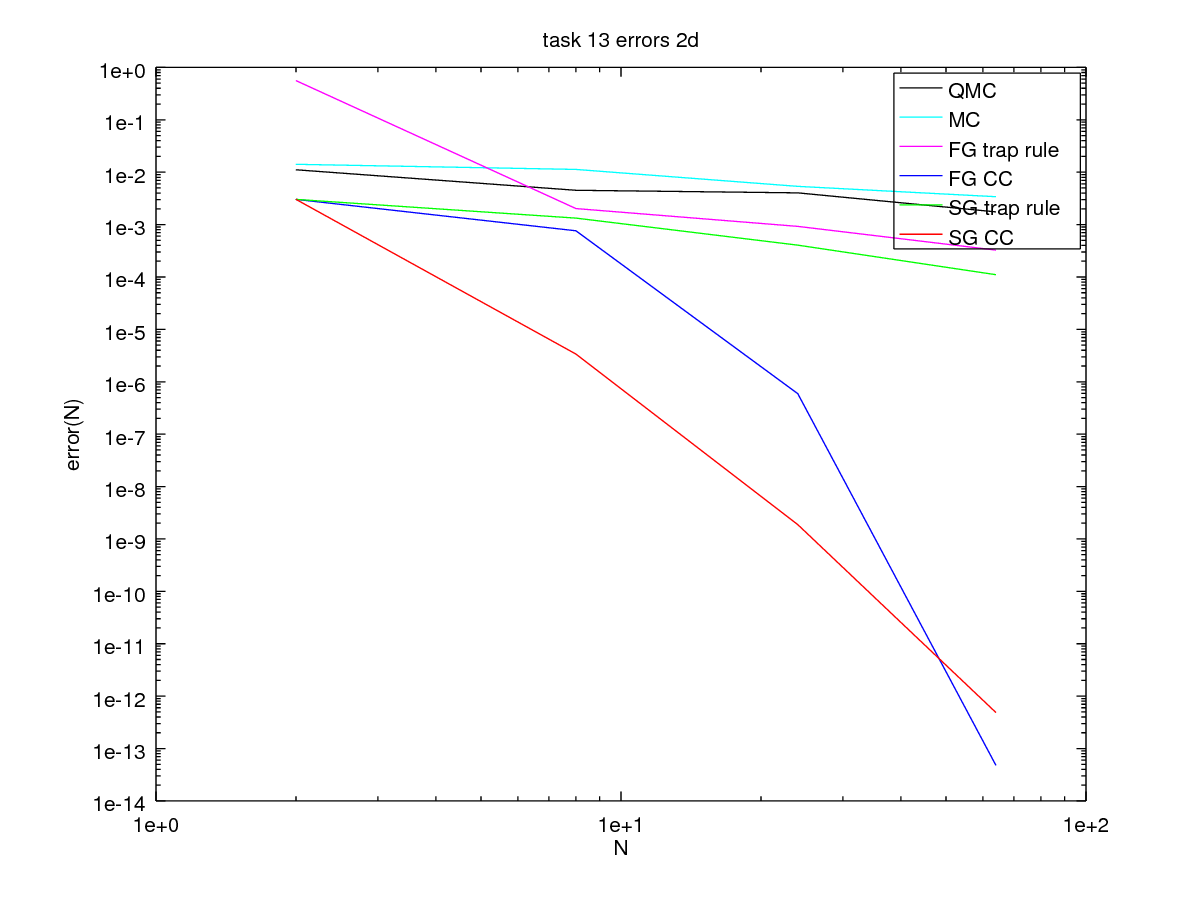
\includegraphics[scale=0.5]{task_13_d2.png}
\end{center}
\begin{center}
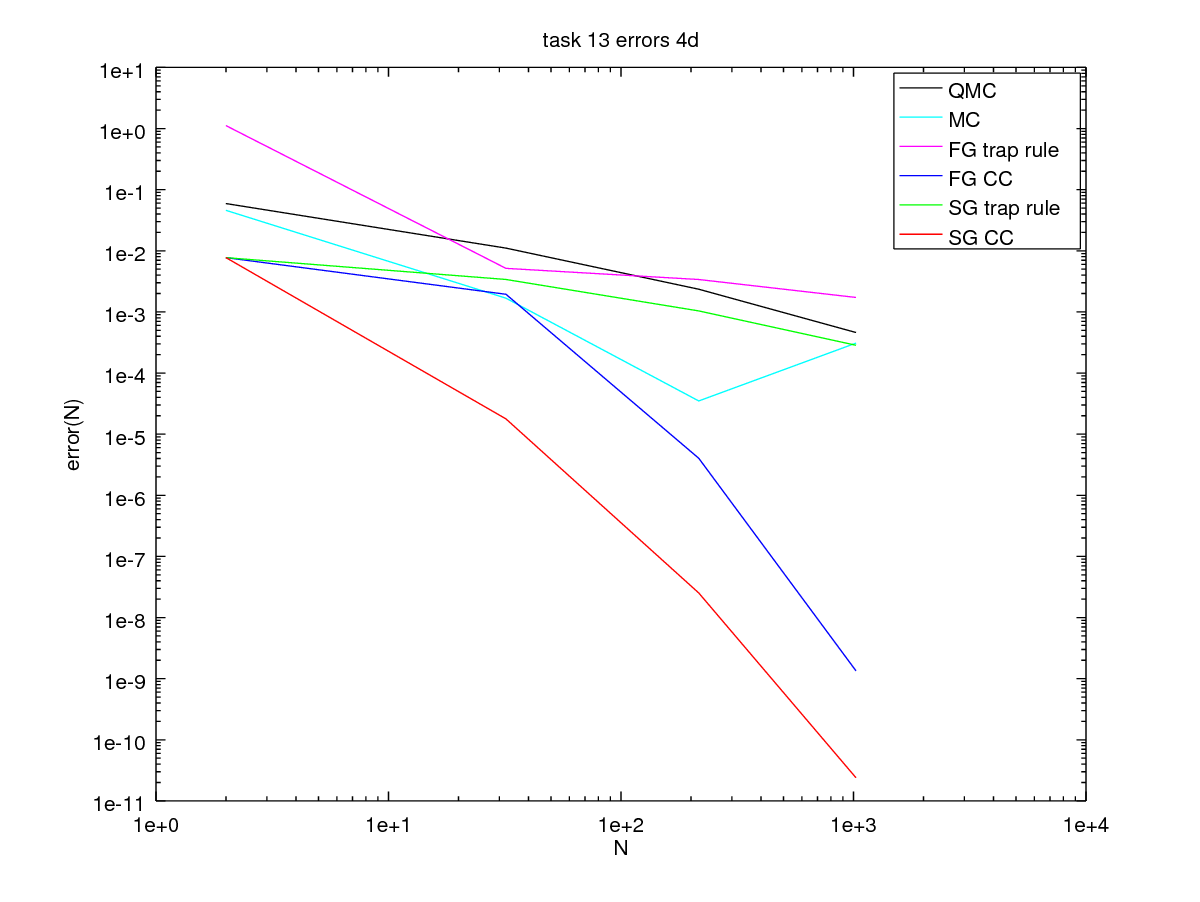
\includegraphics[scale=0.5]{task_13_d4.png}
\end{center}
\begin{center}
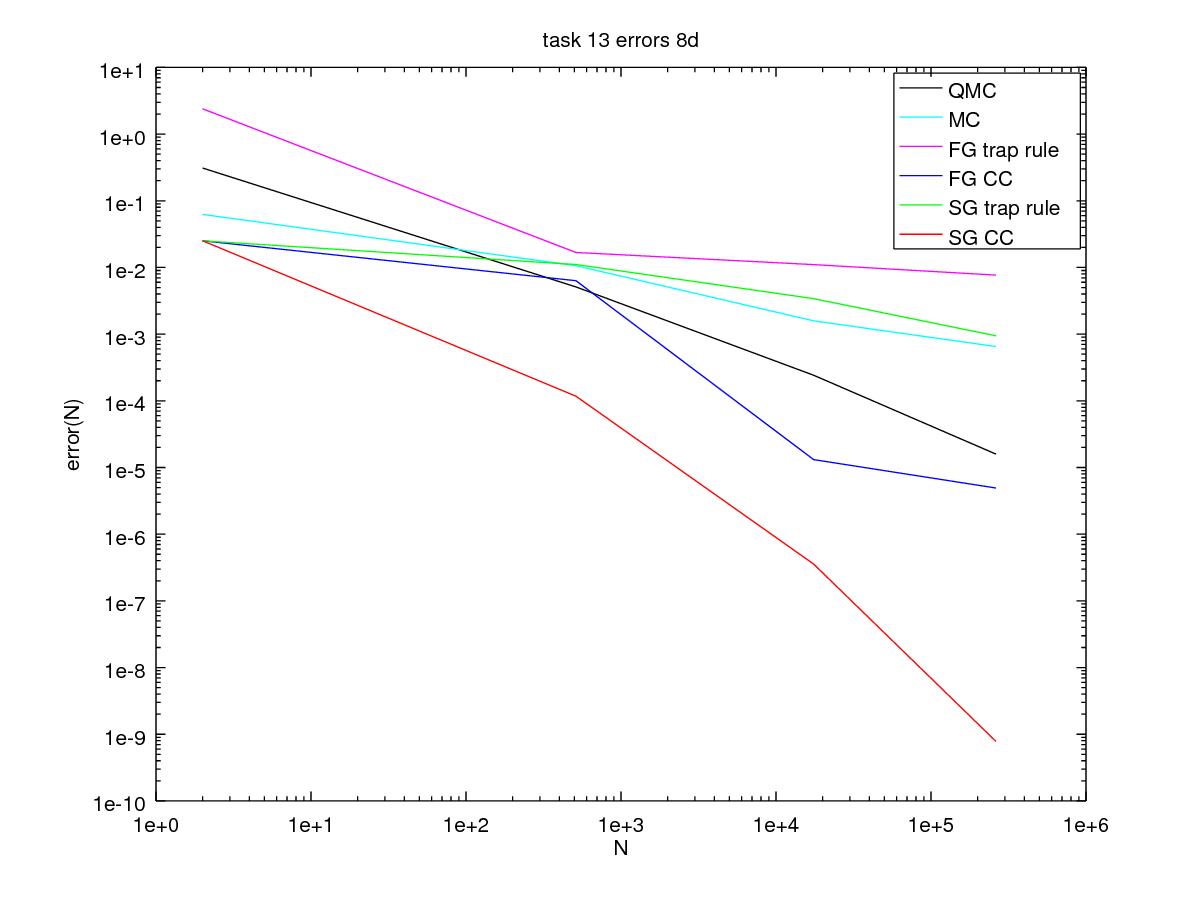
\includegraphics[scale=0.5]{task_13_d8.png}
\end{center}
Obviously, the Sparse Grid Method has the best convergence and the Full
Grid method has the second best convergence, while MC and QMC can't match
these convergence rates. Since the quadrature nodes are better distributed on
the integration region, QMC has better convergence than MC.

\section*{Task 15}
\begin{center}
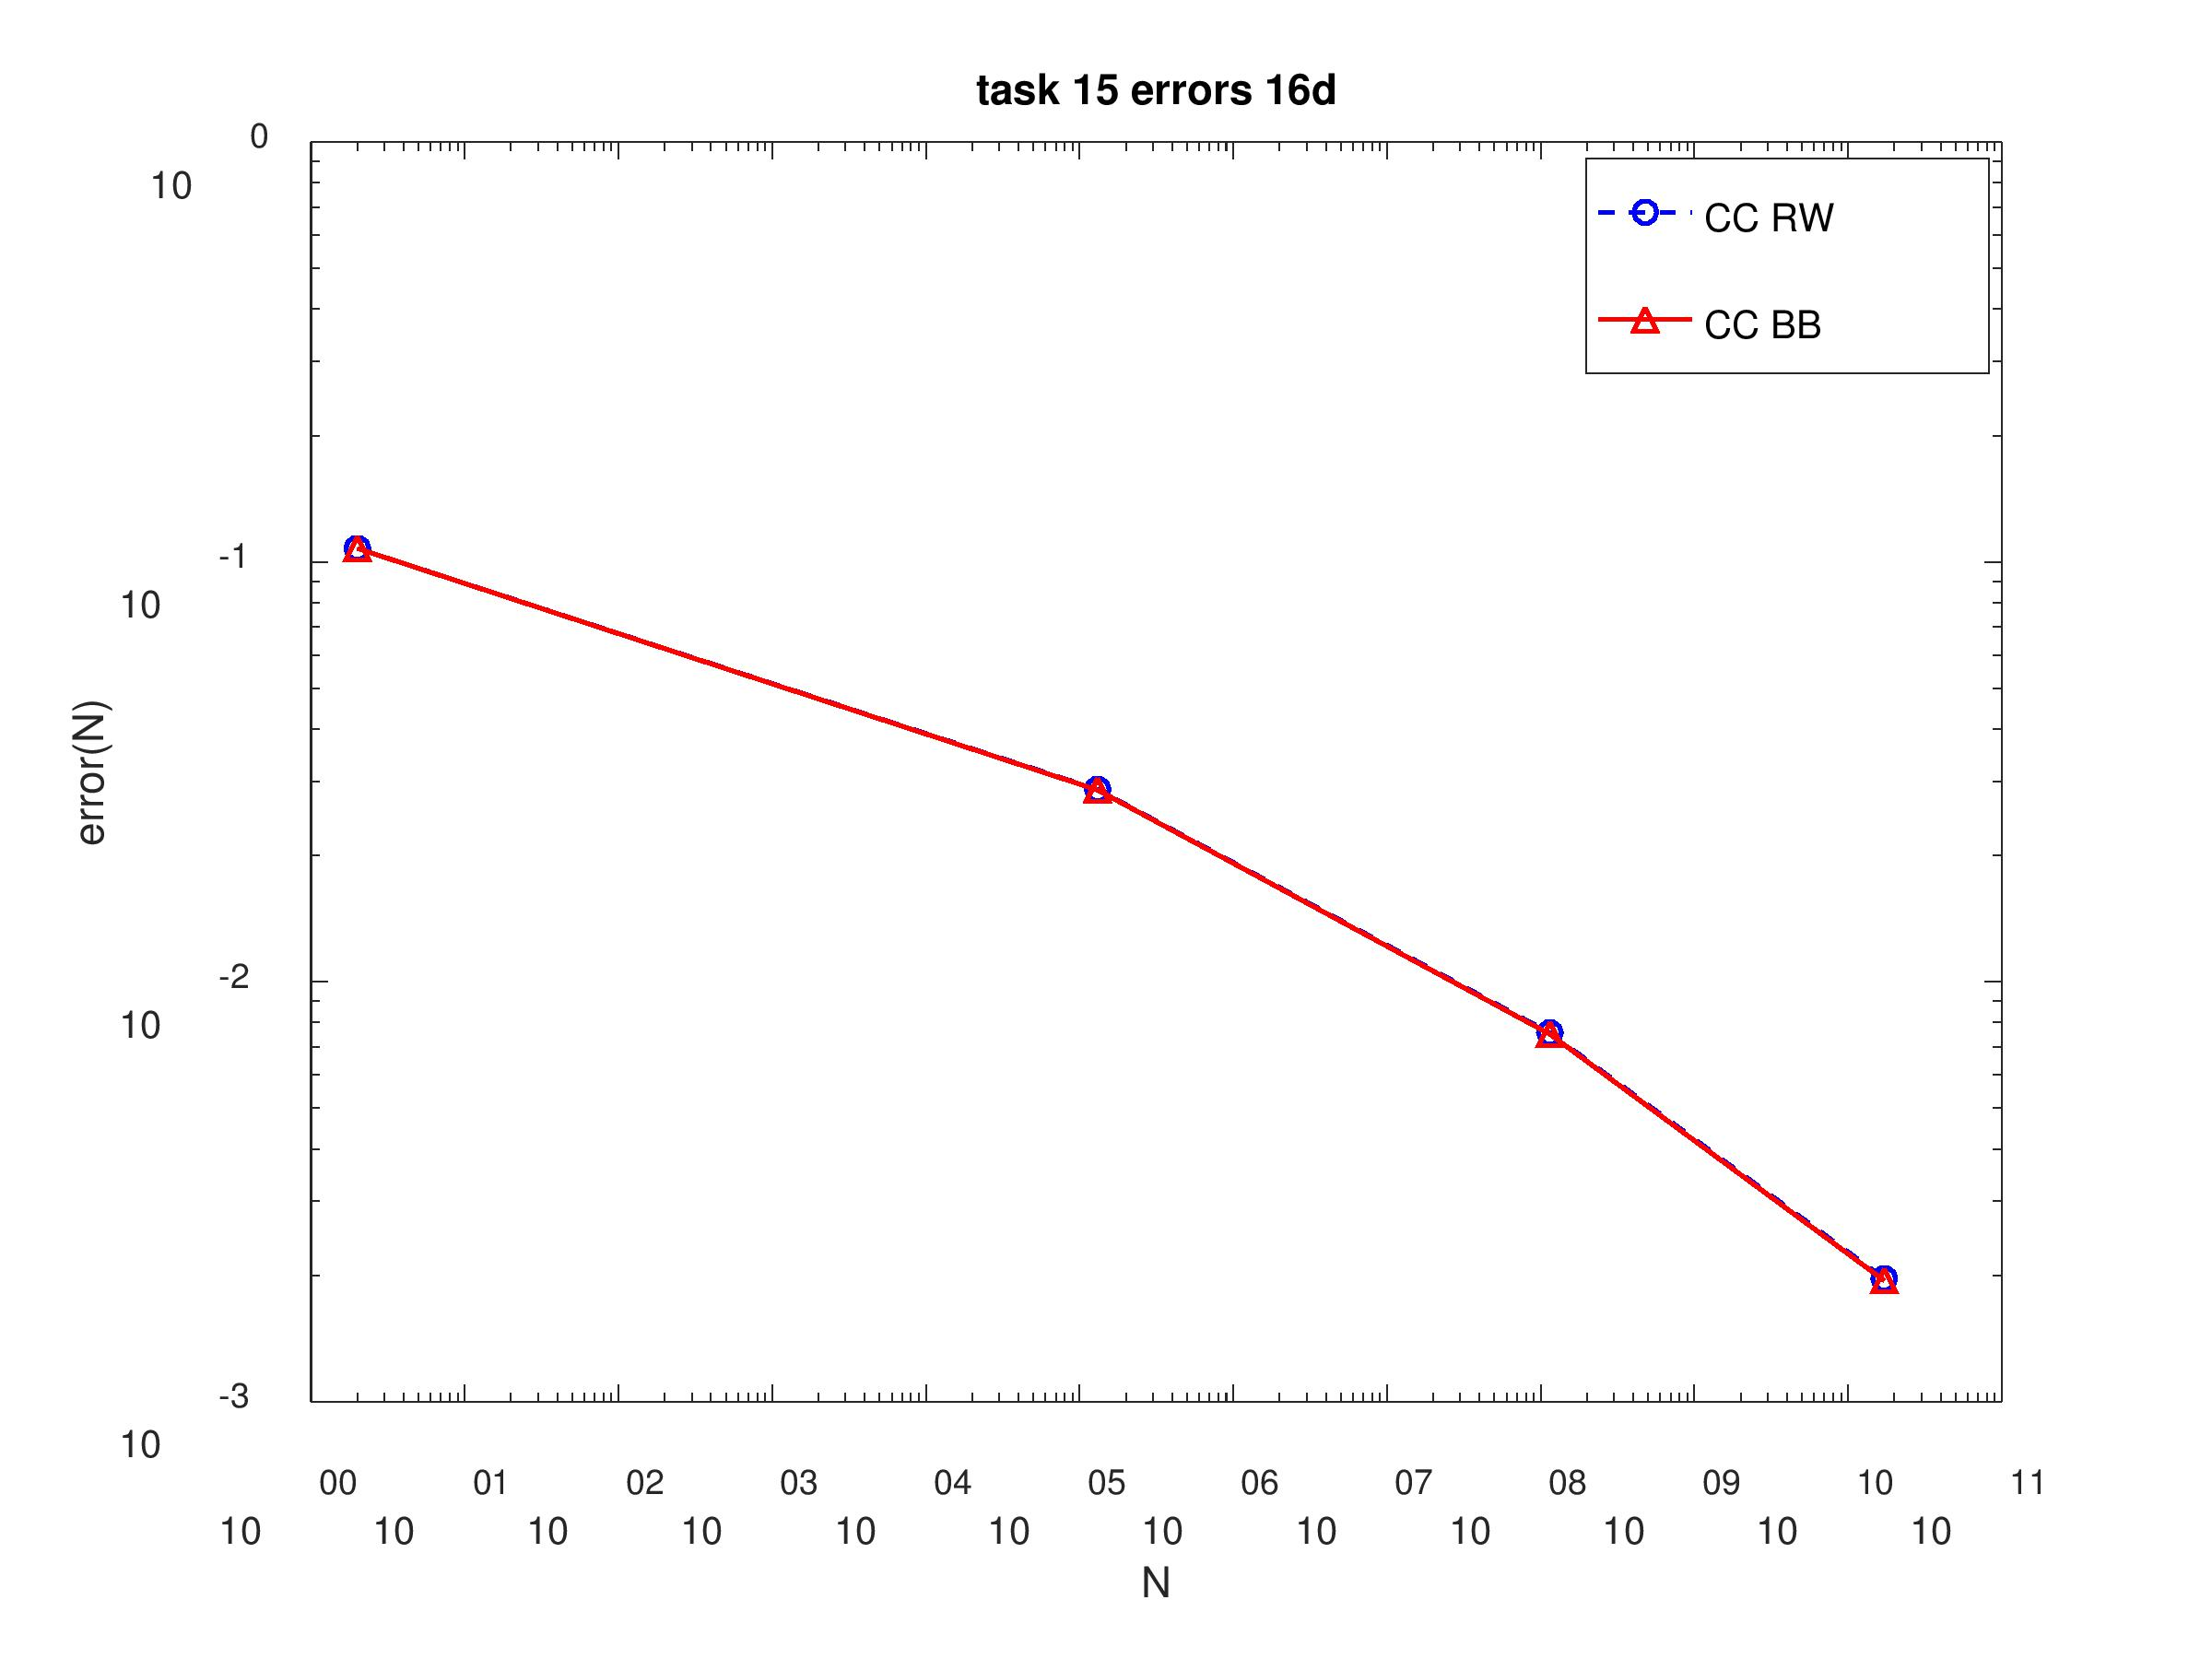
\includegraphics[scale=0.29]{task15.png}
\end{center}
\section*{Task 16}
\begin{center}
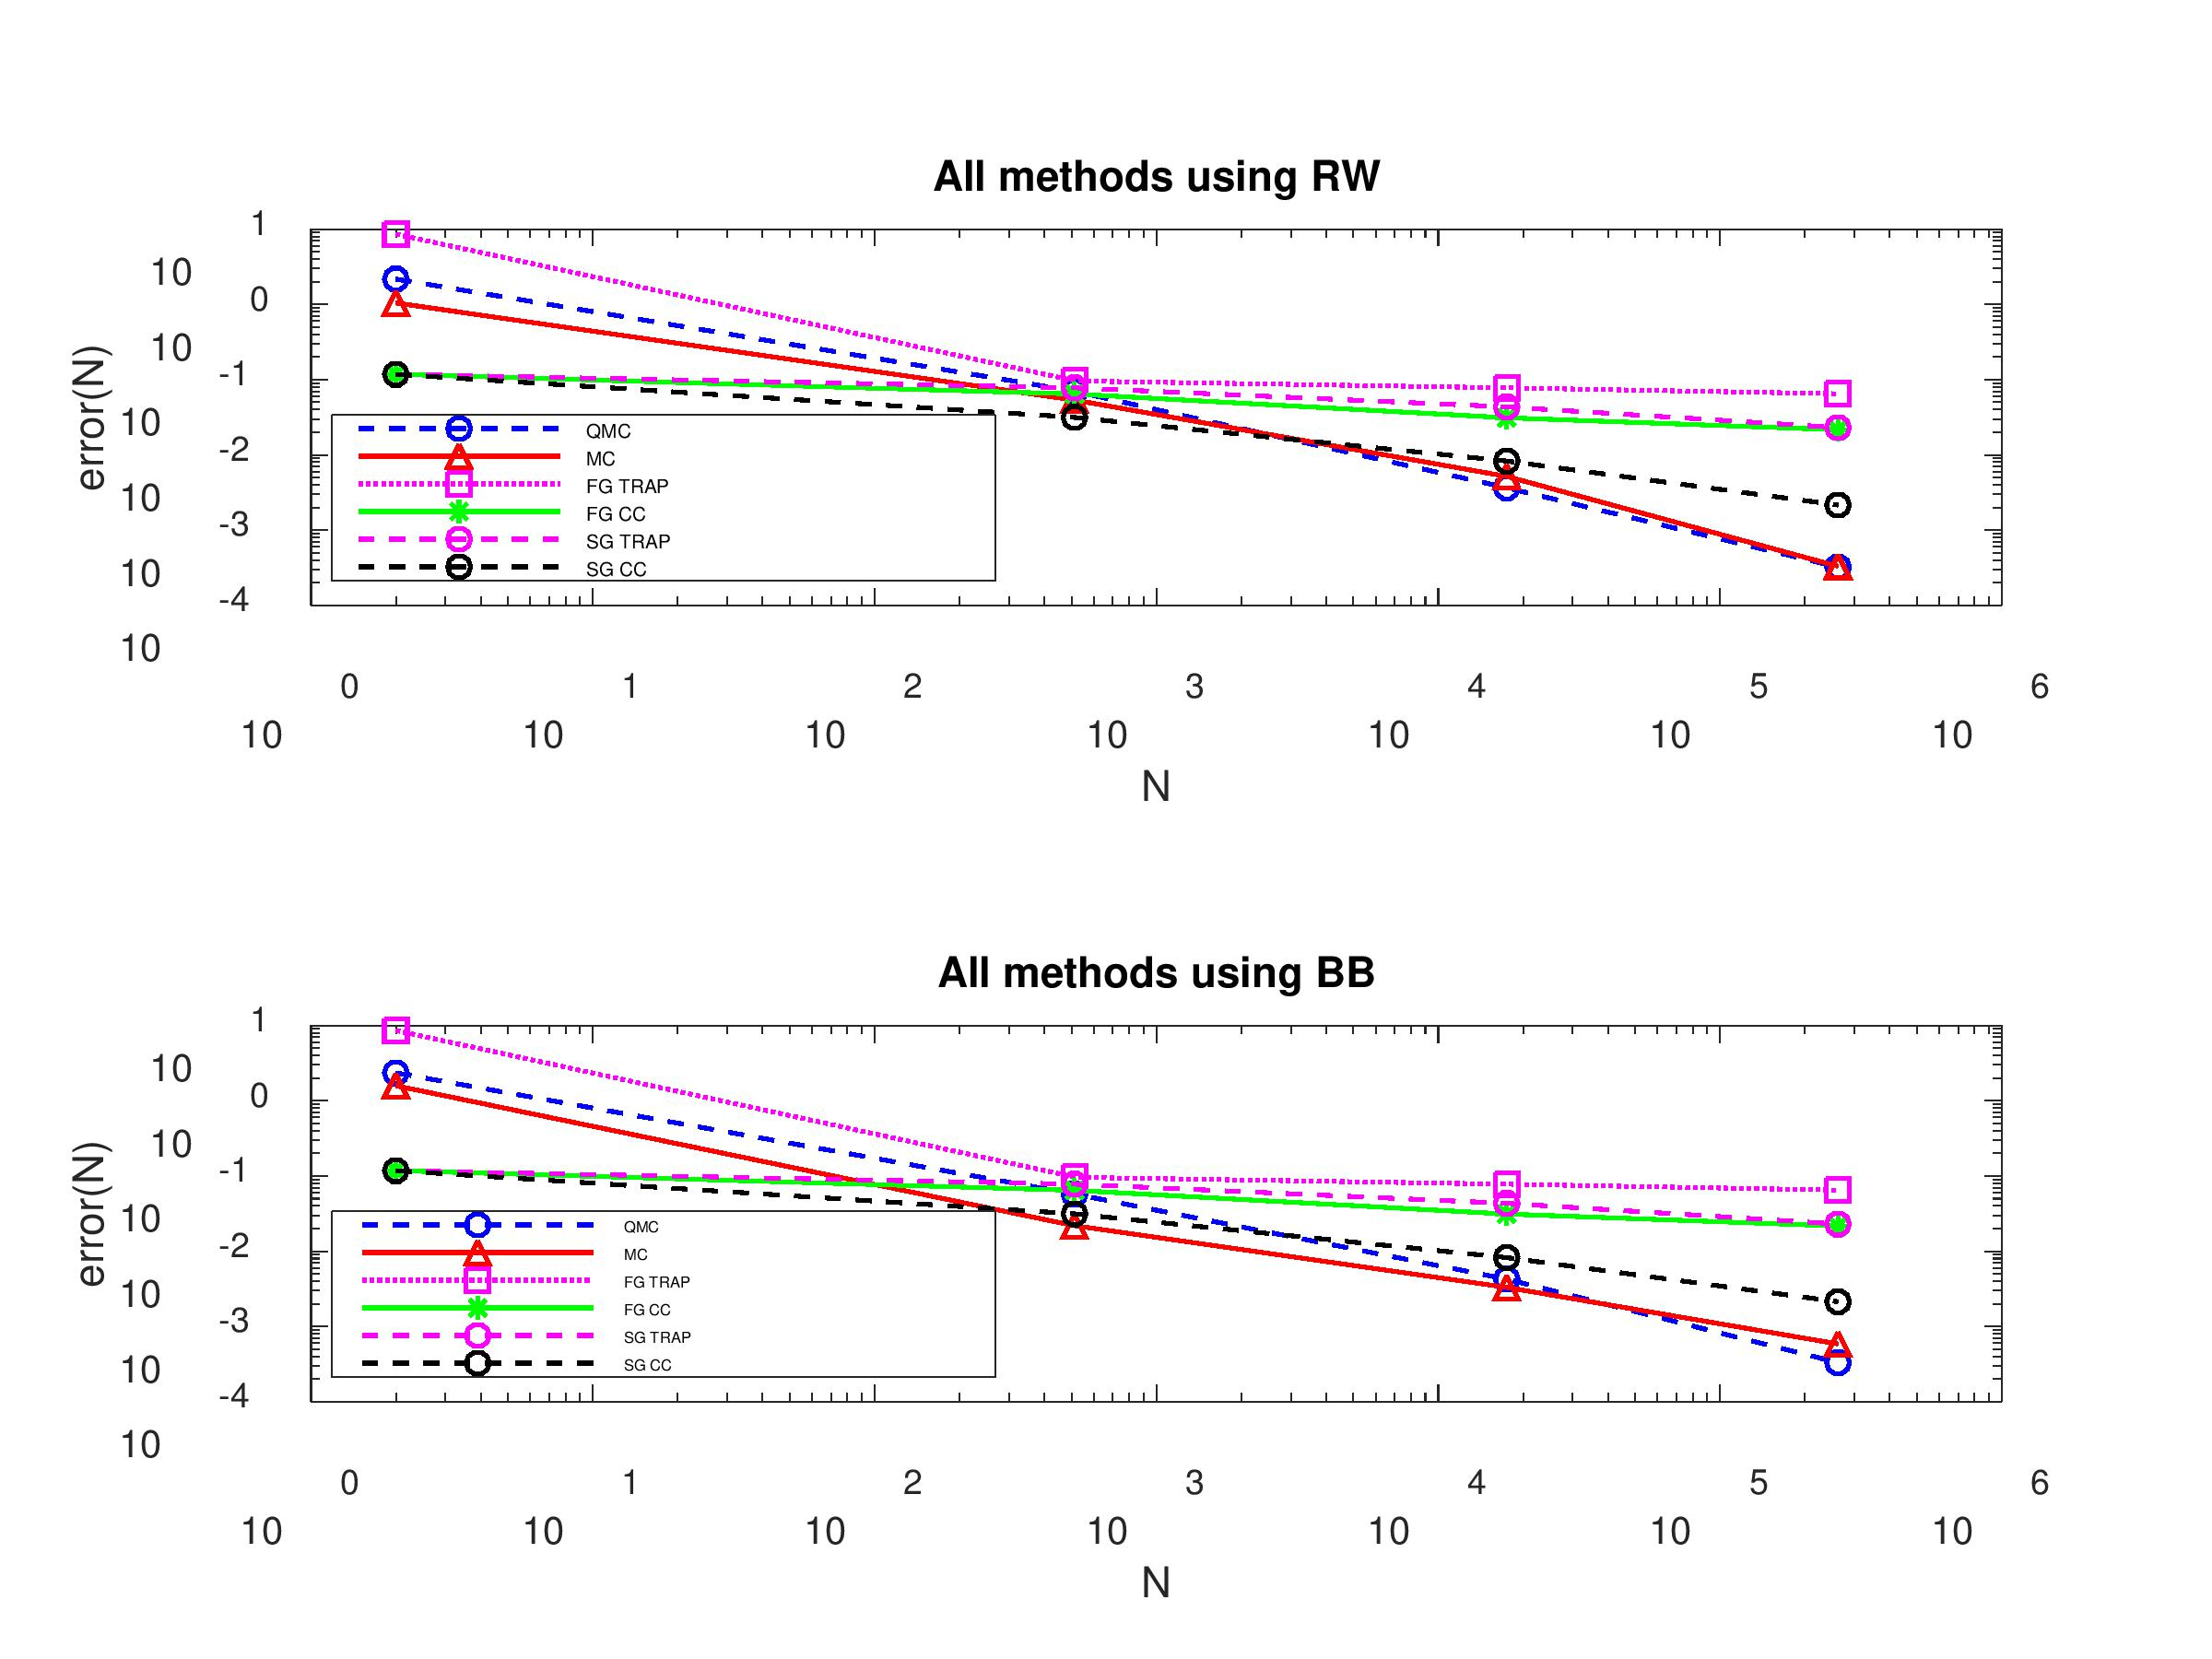
\includegraphics[scale=0.3]{task16.png}
\end{center}
Again, Brownian Bridge has better convergence than Random Walk. 
\section*{Task 17}
\begin{center}
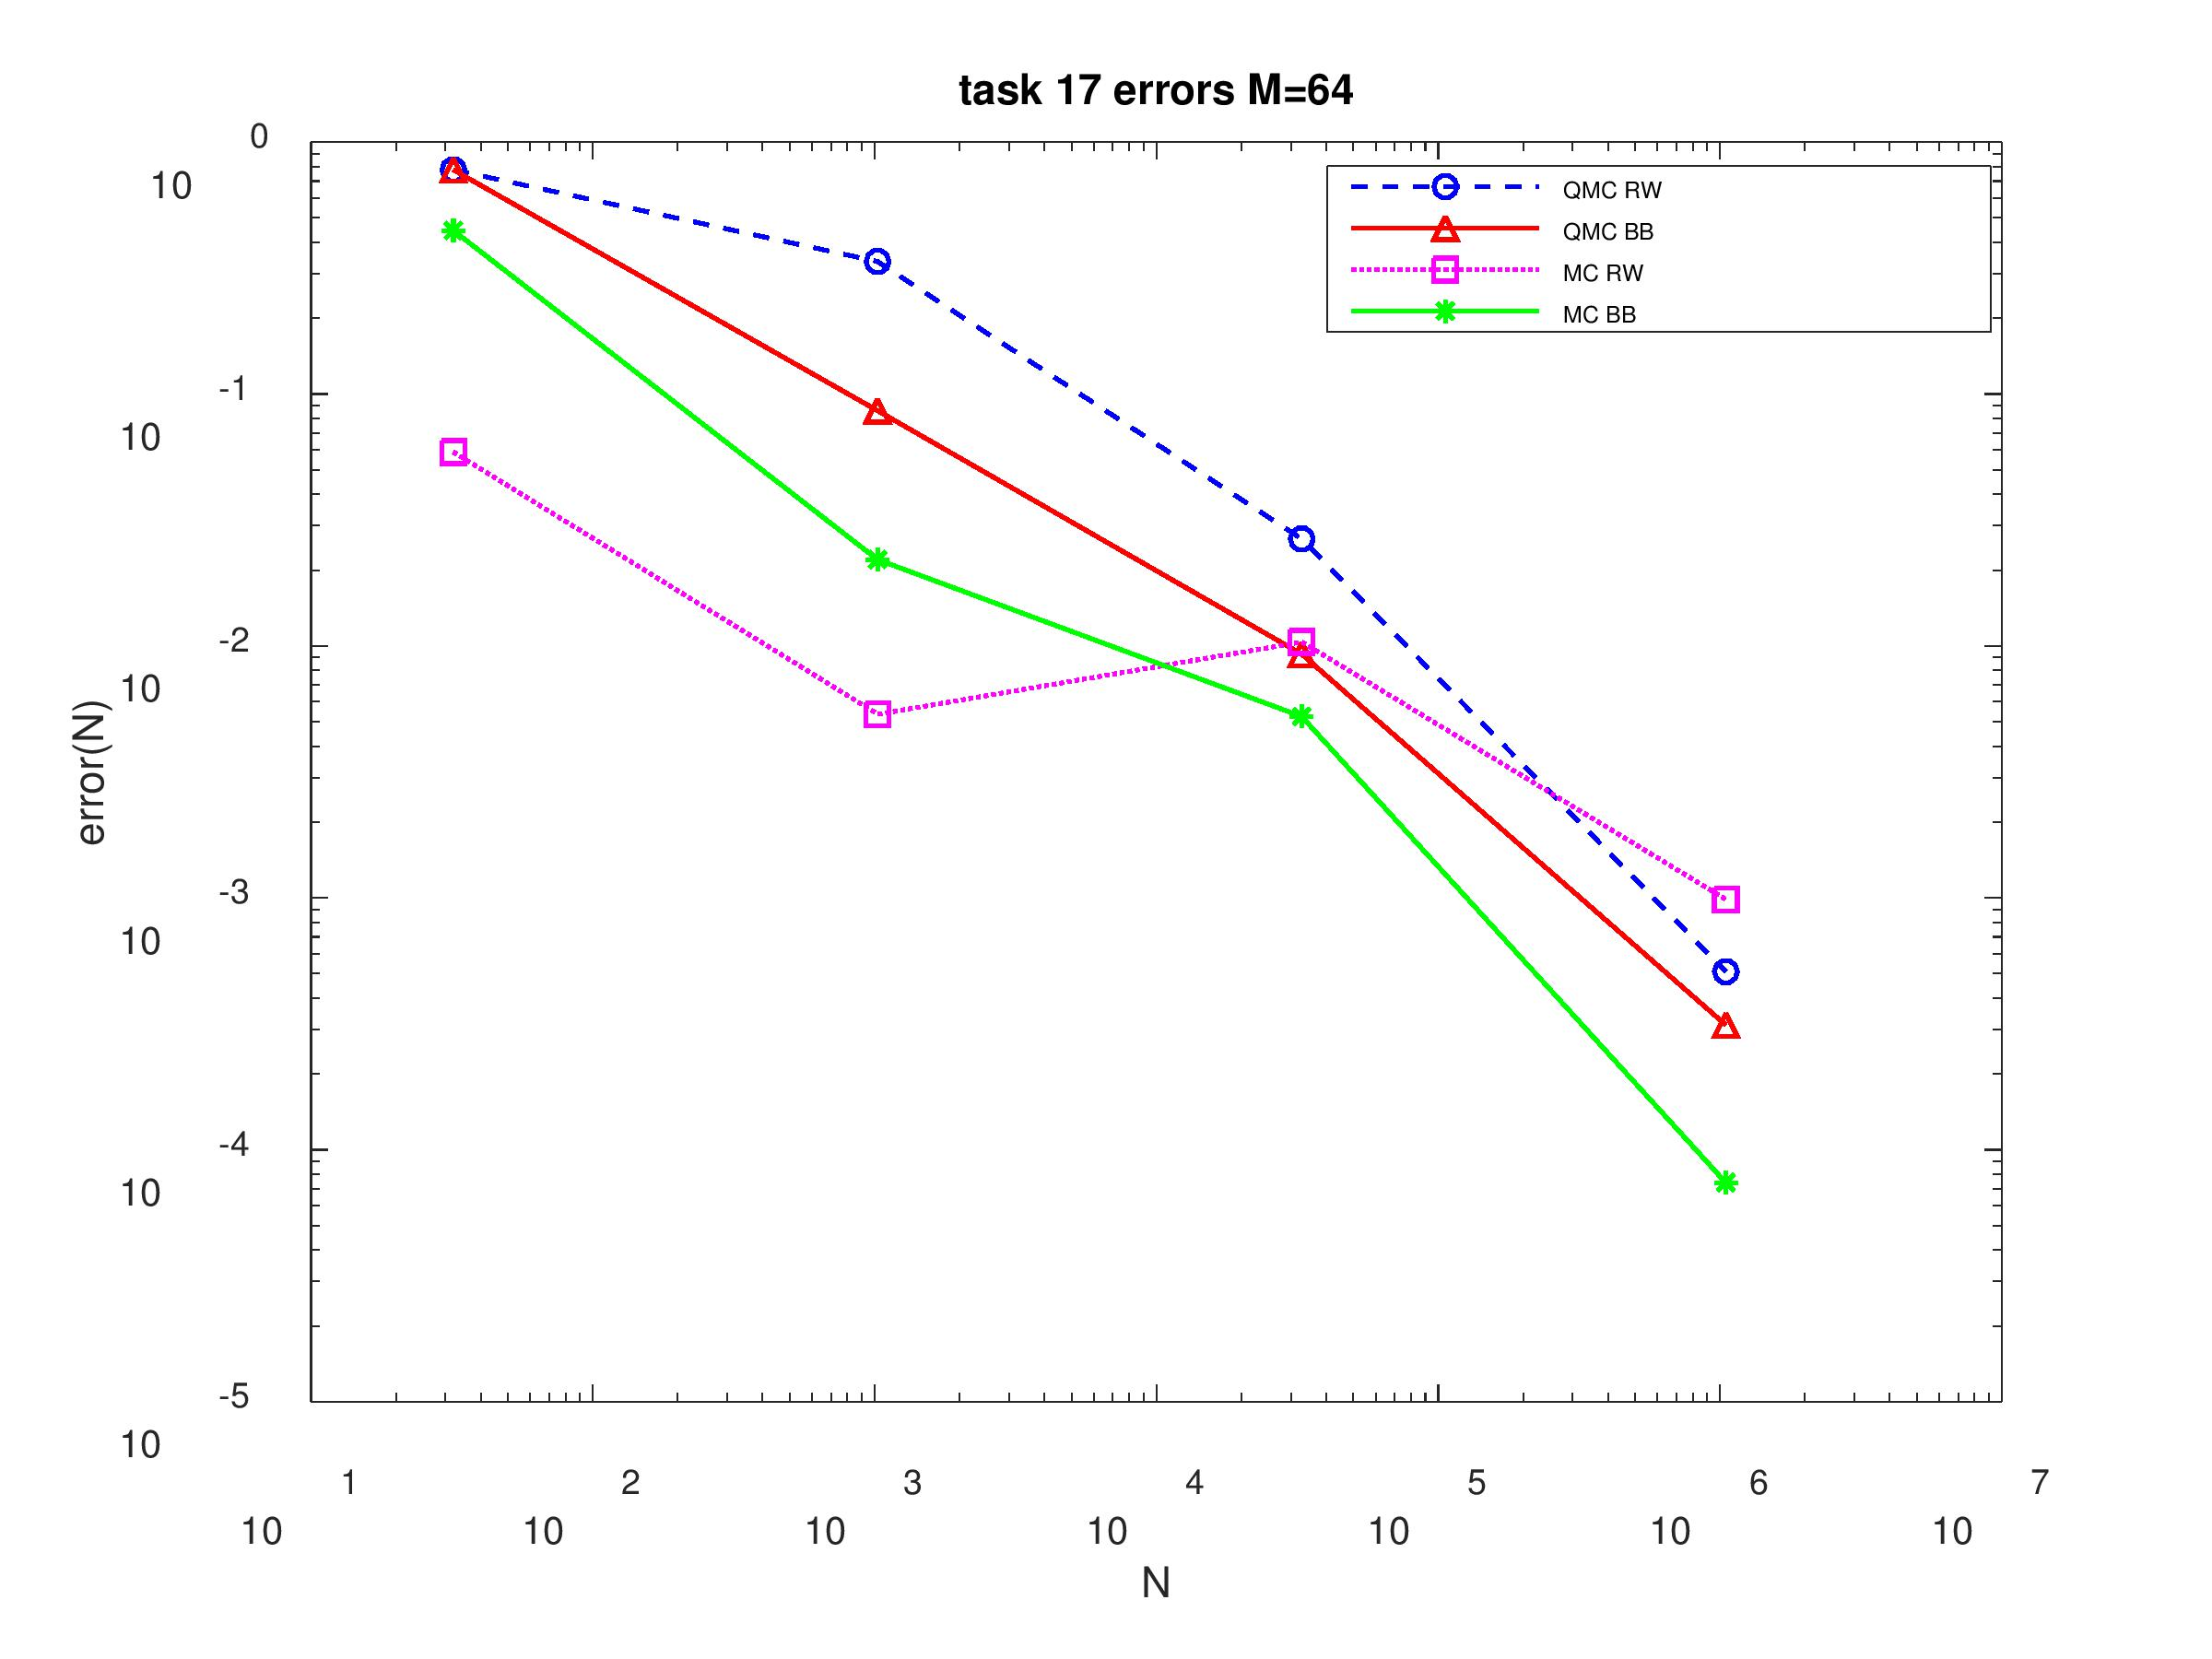
\includegraphics[scale=0.28]{task17.png}
\end{center}
This again illustrates the superiority of Brownian Bridge Interpolation over
Random Walk. Furthermore, the simpler MC method has almost the same
convergence as QMC.

\section*{Task 18}

The difference between MC and QMC is, that MC uses actual pseudo random numbers, while QMC uses deterministic sequences. For this reason, QMC Quadrature Nodes are more evenly distributed over the integration region, which enhances the convergence rate of QMC (which is $\mathcal{O}(N)$) compared to the convergence of $\mathcal{O}(N^{1/2})$ of Monte Carlo Method. However, there is a higher computational effort in creating quasi-random-number sequences, which increases the cost of QMC especially in high dimensions compared to Monte Carlo. \\

Both, QMC and MC, can integrate a wide range of functions, regardless of how smooth these functions are. \\

Sparse Grids and Full Grids make use of nodes and weights which result from quadrature methods like Clenshaw-Curtis or Trapezoidal rule. These methods can only be applied to somewhat smoother functions, but they have much better convergence rates. 
Full Grids are heavily affected by the dimension, with the number of nodes increasing exponentially with increasing dimension. For sparse grids, dependence on dimension is considerably lower. \\

Therefore, if it is known that the integrand will be relatively smooth, using Sparse Grid methods is the best way to compute integrals in high dimensions. However, if the integrand is unknown or if the integrand is a function that is not differentiable in many points, MC and QMC integration are the preferred methods, espacially in high dimensions.

\end{document}

